\section{Implementation}\label{impl}
This section presents an overview of the implementation of SCache. 
% {\color{red}
% Here we use Spark as an example of DAG framework to illustrate the work flow of shuffle optimization. 
% We will first present the system overview in Subsection \ref{arch} while the following two subsections focus on the two constraints on memory management.
% }
{\color{blue}
We first present the system overview and the detail of sampling in Subsection \ref{arch}. 
The following \ref{memorymanage} subsection focuses on two constraints on memory management.
In Subsection \ref{crossframework}, we evaluate the cross-framework capability of SCache. 
At last, we discuss the cost of adapting SCache and fault tolerance. 
}


\subsection{System Overview}\label{arch}
SCache consists of three components: a distributed shuffle data management system, a DAG co-scheduler, and a %{\color{red}daemon inside Spark.}
{\color{blue} worker daemon. As a plug-in system, SCache needs to rely on a DAG framework.} As shown in Figure \ref{fig:architecture}, SCache employs the legacy master-slaves architecture like GFS \cite{gfs} for the shuffle data management system. 
The master node of SCache coordinates the shuffle blocks globally with application context. The worker node reserves memory to store blocks.
The coordination provides two guarantees: (a) data is stored in memory before tasks start and (b) data is scheduled on-off memory with all-or-nothing and context-aware constraints. 
The daemon bridges the communication between %{\color{red}Spark}
{\color{blue} DAG framework} and SCache. The co-scheduler is dedicated to pre-schedule reduce tasks with DAG information and enforce the scheduling results to %{\color{red}Spark scheduler}
 {\color{blue} the original scheduler in framework}.

% SCache consists of three components: a distributed shuffle data management system, a DAG co-scheduler, and a {\color{blue} worker daemon}. As shown in Figure \ref{fig:arch}, SCache employs the legacy master-slaves architecture like GFS \cite{gfs} for shuffle data management system. 

% The master node of SCache coordinates the shuffle blocks globally with application context. The worker node reserves memory to store blocks.
% The coordination provides two guarantees: (a)data is stored in memory before tasks start and (b)data is scheduled on-off memory with all-or-nothing and context-aware constraints. 
% The daemon bridges the communication between {\color{blue}DAG framework} and SCache. The co-scheduler is dedicated to pre-schedule reduce tasks with DAG information and enforce the scheduling results to {\color{blue} original scheduler in framework master}.

% {\color{red}
% When a Spark job starts, the DAG will be first generated. 
% During the DAG generation, the shuffle dependencies among Resilient Distributed Datasets (RDDs) will then be submitted through the daemon process in Spark driver. 
% }
{\color{blue}
When a DAG job is submitted, the DAG information is generated in framework task scheduler. 
Before the computing tasks begin, the shuffle dependencies are determined based on DAG.
}
For each shuffle dependency, the shuffle ID, the type of partitioner, the number of map tasks, and the number of reduce tasks are included.  If there is a specialized partitioner, such as range partitioner, in the shuffle dependencies, the daemon will insert a sampling application before the {\color{blue}computing job}. We will elaborate the sampling procedure in the Section \ref{sampling}.
% \begin{minipage}{\columnwidth}
% \begin{algorithm}[H]
% \caption{Heuristic MinHeap Scheduling for Single Shuffle}
% \label{hminheap}
% 	\begin{algorithmic}[1]
% 	\small
% 	\Procedure{\Large schedule}{$m, host\_ids, p\_reduces$}
% 		\State $m\gets$ partition number of map tasks
% 		\State $R\gets$ sort $p\_reduces$ by size in descending order
% 		\State $M\gets$ min-heap $\left\{ host\_id \rightarrow \left( \left[ reduces \right], size \right) \right\}$
% 		\State $idx\gets$ len$\left(R\right) - 1$
% 		\While{$idx \geq 0$}
% 		\Comment{Schedule reduces by MinHeap}
% 		\State $M\left[0\right].size \mathrel{+}= R\left[idx\right].size$
% 		\State $M\left[0\right].reduces.append\left(R\left[idx\right]\right)$
% 		\State $R\left[idx\right].assigned\_host \gets M \left[0\right].host\_id$
% 		\State Sift down $M\left[0\right]$ by $size$
% 		\State $idx\gets idx-1$
% 		\EndWhile
% 		\State $max\gets$ maximum size in $M$
% 		\State Convert $M$ to mapping $\left\{ host\_id \rightarrow \left( \left[ rid\_arr \right], size \right) \right\}$
% 		\ForAll{$reduce$ in $R$}
% 		\Comment{Heuristic swap by locality}
% 			\If{$reduce.assigned\_id \neq reduce.host\_id$}
% 				\State $p\gets reduce.prob$
% 				\State $norm\gets \left(p-1/m\right)/\left(1-1/m\right)/10$
% 				\State $upper\_bound \gets \left(1 + norm\right) \times max$
% 				\State SWAP\_TASKS$\left(M, reduce, upper\_bound\right)$
% 			\EndIf
% 		\EndFor
% 		% \Comment{$m$ is the number of input data}
% 		% \Comment{$r$ is partition number of reduces}
% 		% \Comment{$hosts$ is array of (hostid, partitionids[], size)}
% 		% \Comment{$c$ is $r*m$ array of composition data}
% 		% \Comment{$pSize$ is $r$ size array of predicted size of reduces}
% 		\Return $M$
% 	\EndProcedure
% 	\Procedure{\Large swap\_tasks}{$M, reduce, upper\_bound$}
% 		\State $reduces \gets M\left[reduce.host\_id\right].reduce$	
% 		\State $candidates \gets$ Select from $reduces$ that $assigned\_id \neq host\_id$ \textbf{and} total size closest to $reduce.size$
% 		\State $\Delta size \gets sizeOf\left(candidates\right) - reduce.size$
% 		\State $size\_host \gets M\left[reduce.host\_id\right].size - \Delta size$
% 		\State $size\_assigned \gets M\left[reduce.assigned\_id\right].size + \Delta size$
% 		\If{$size\_host\leq upper\_bound$ \textbf{and} \\
% 			\qquad \; $size\_assigned\leq upper\_bound$}
% 			\State Swap $candidates$ and $reduce$
% 			\State Update $size$ in $M$
% 			\State Update $assigned\_host$ in $candidates$ and $reduce$
% 		\EndIf
% 	\EndProcedure
% 	\end{algorithmic}
% \end{algorithm}
% \end{minipage}

When a map task finishes computing, the shuffle write implementation of the DAG framework is modified to call the SCache API and move all the blocks out of {\color{blue}framework worker} through memory copy. 
After that, the slot will be released (without being blocked on disk operations).
When a block of the map output (i.e., "map output" in Figure \ref{fig:shuffle}) is received, the SCache worker will send the block ID and the size to the master.
If the collected map output data reach the observation threshold, the DAG co-scheduler will run the scheduling Algorithm \ref{hminheap} or \ref{mhminheap} to pre-schedule the reduce tasks and then broadcast the scheduling result to start pre-fetching on each worker.
% After that, when a map task is finished, each node will receive a broadcast message. 
SCache worker will filter the reduce tasks' IDs that are scheduled on itself and start pre-fetching shuffle data from the remote. 
% {\color{red}
% To enforce SCache pre-scheduled tasks -- node mapping, we insert some lines of codes in Spark DAG Scheduler.
% For RDDs with shuffle dependencies, Spark DAG scheduler will consult SCache master to get the preferred location for each partition and set \textit{NODE\_LOCAL} locality level on corresponding reduce tasks.
% }
{\color{blue}
In order to force the DAG framework to run according to the SCache pre-scheduled results, we insert some lines of codes in framework scheduler.
After modification, the DAG scheduler consults SCache co-scheduler to get the preferred location for each task.
}
% In the case of extreme skew scenario, such as Figure \ref{fig:range_pre_sample}, Heuristic MinHeap trades about 0.05\% percent of stage completion time for 99\% reduction of shuffle data transmission through network by heuristicly swapping tasks.
% \begin{minipage}{\columnwidth}
% \begin{algorithm}[H]
% \caption{Accumulate Heuristic Scheduling for Multi-Shuffles}
% \label{mhminheap}
% 	\begin{algorithmic}[1]
% 	\small
% 	\Procedure{\Large m\_schedule}{$m, host\_id, p\_reduces, shuffles$}
% 		\State $m\gets$ partition number of map tasks
% 		\Comment $shuffles$ is the previous schedule result 
% 		\ForAll{$r$ in $p\_reduces$}
% 			\State $r.size \mathrel{+}= shuffles\left[r.rid\right].size$
% 			\If{$shuffles\left[r.rid\right].size\geq r.size \times r.prob$}
% 				\State $r.prob\gets shuffles\left[r.rid\right].size / r.size$
% 				\State $r.host\_id\gets shuffles\left[r.rid\right].assigned\_host$
% 			\EndIf
% 		\EndFor
% 		\State $M\gets$ $SCHEDULE\left(m, host\_id, p\_reduces\right)$
% 		\ForAll{$host\_id$ in $M$}
% 			\Comment Re-shuffle
% 			\ForAll{$r$ in $M\left[host\_id\right].reduces$}
% 				\If{$host\neq shuffles\left[r.rid\right].assigned\_host$}
% 				\State Re-shuffle data to $host$
% 				\State $shuffles\left[r.rid\right].assigned\_host\gets host$
% 				\EndIf
% 			\EndFor
% 		\EndFor
% 		\Return $M$
% 	\EndProcedure
% 	\end{algorithmic}
% \end{algorithm}
% \end{minipage}

\subsubsection{Reservoir Sampling}\label{sampling}
If the submitted shuffle dependencies contained a RangePartitioner or a customized non-hash partitioner, {\color{blue}the SCache master will send a sampling request to the framework master}. 
The sampling job uses a reservoir sampling algorithm \cite{reservoir} on each partition. 
For the sample number, it can be tuned to balance the overhead and accuracy. 
The sampling job randomly selects some items and performs a local shuffle with the partitioner (see Figure \ref{fig:sample}). 
At the same time, the items number is counted as the weight. 
These sampling data will be aggregated by reduce task ID on SCache master to predict the reduce partition size. 
After the prediction, SCache master will call Algorithm \ref{hminheap} or \ref{mhminheap} to do the pre-scheduling.

% \begin{figure}
% 	\centering
% 	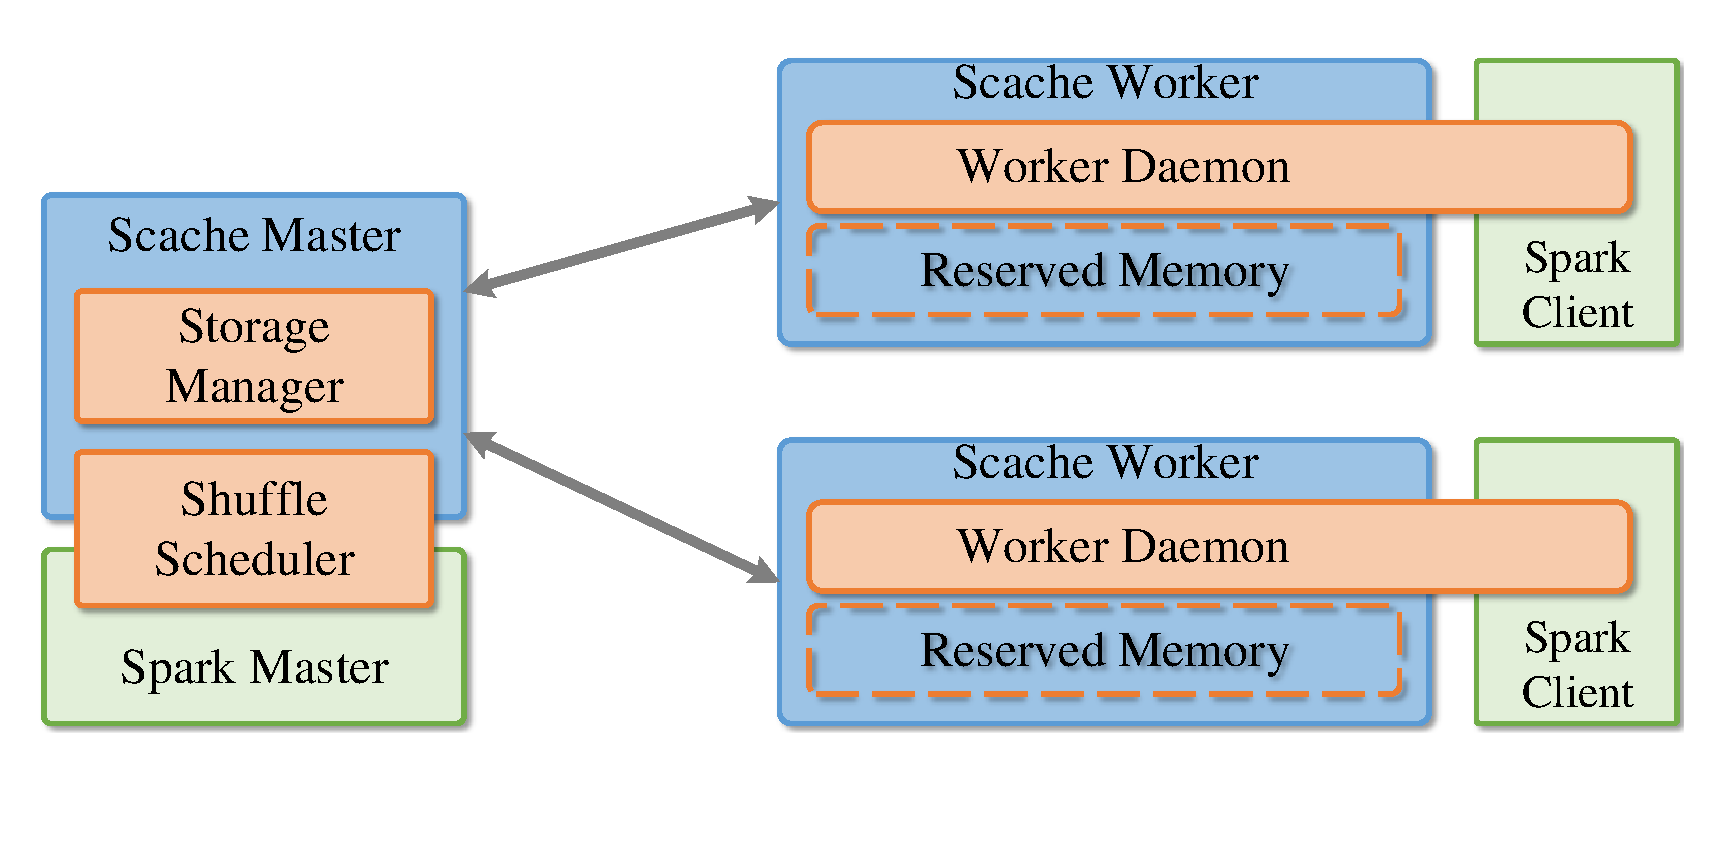
\includegraphics[width=0.8\linewidth]{fig/arch}
% 	\caption{\color{red}SCache Architecture}
% 	\label{fig:arch}
% 	\vspace{-0.5em}
% \end{figure}

\begin{figure}
	\centering
	\begin{minipage}{.4\textwidth}
		\centering
		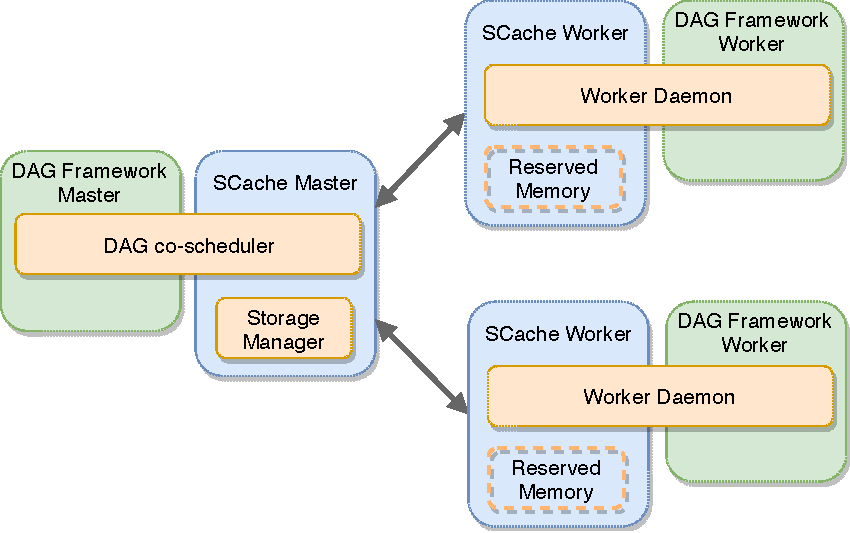
\includegraphics[width=\linewidth]{fig/architecture}
		\caption{\color{blue}SCache Architecture}
		\label{fig:architecture}
		% \vspace{-0.5em}
	\end{minipage}\hfill
	\begin{minipage}{.4\textwidth}
		\centering
		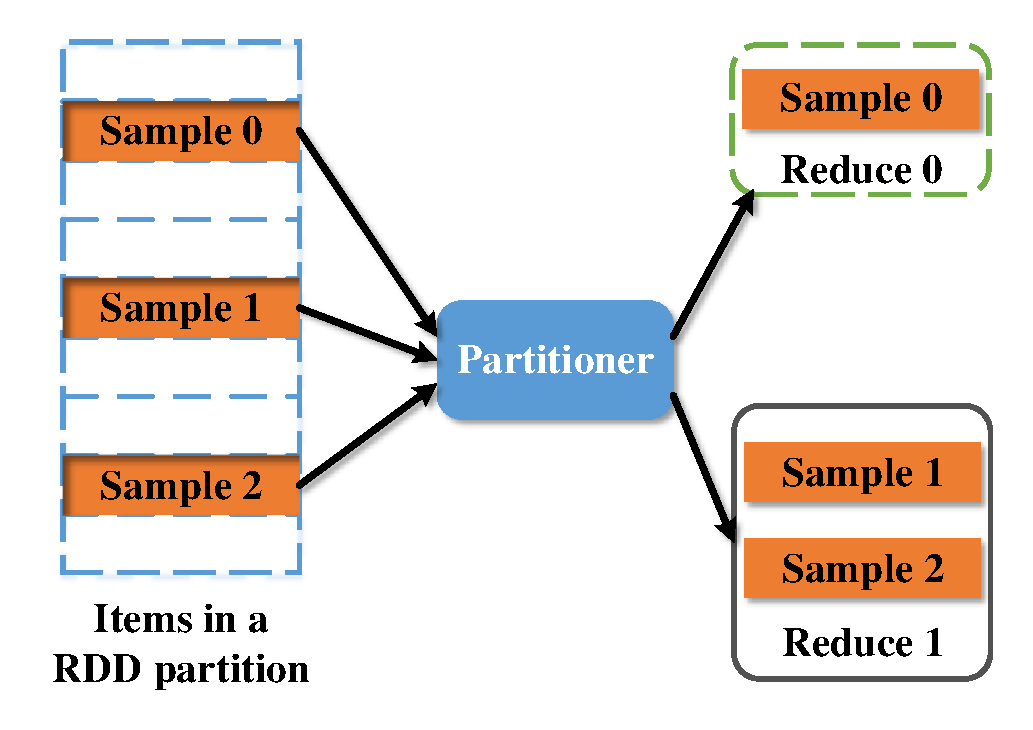
\includegraphics[width=\linewidth]{fig/sample}
		\caption{Reservoir Sampling of One Partition}
		\label{fig:sample}
		% \vspace{-1em}
	\end{minipage}
\end{figure}

\subsection{Memory Management}\label{memorymanage}
As mentioned in Section \ref{observation}, though the shuffle size is relatively small, memory management should still be cautious enough to limit the effect of performance of DAG framework.
When the size of cached blocks reaches the limit of reserved memory, SCache flushes some of them to the disk temporarily, and re-fetches them when some cached shuffle blocks are consumed or pre-fetched. 
To achieve the maximum overall improvement, SCache leverages two constraints to manage the in-memory data-all-or-nothing and context-aware-priority.



\subsubsection{All-or-Nothing Constraint}
This acceleration of in-memory cache of a single task is necessary but insufficient for a shorter stage completion time. 
Based on the observation in Section \ref{multi}, in most cases one single stage contains multi-rounds of tasks. 
If one task missed a memory cache and exceeded the original bottleneck of this round, that task might become the new bottleneck and then slow down the whole stage. 
PACMan \cite{pacman} has also proved that for multi-round stage/job, the completion time improves in steps when $n\times number\ of\ tasks\ in\ one\ round$ of tasks have data cached simultaneously. 
Therefore, the cached shuffle blocks need to match the demand of all tasks in one running round at least. We refer to this as the all-or-nothing constraint.

According to all-or-nothing constraint, SCache master leverages the pre-scheduled results to determine the bound of each round, and sets blocks of one round as the minimum unit of storage management.
For those incomplete units, SCache marks them as the lowest priority.
% Following the all-or-noting constraint can maximum the improvement in stage completion time by using reserved memory efficiently.

\subsubsection{Context-Aware-Priority Constraint}
Unlike the traditional cache replacement schemes such as MIN \cite{min}, the cached shuffle data will only be used once (without failure), but the legacy cache managements are designed to improve the hit rate.
SCache leverages application context to select victim storage units when the reserved memory is full.

At first, SCache flushes blocks of the incomplete units to disk cluster-widely.
If all the units are completed, SCache selects victims based on two factors --- \textit{inter-shuffle} and \textit{intra-shuffle}.
\begin{itemize}[noitemsep]
	\item Inter-shuffle: SCache master follows the scheduling scheme of Spark to determine the inter-shuffle priority. 
	For example, Spark FIFO scheduler schedules the tasks of different stages according to the submission order. 
	So SCache sets the priorities according to the submission time of each shuffle.
	% For a FAIR scheduler, Spark balances the resource among task sets, which leads to a higher priority for those having more tasks unfinished. 
	% So SCache sets priorities from high to low in a descending order of remaining storage units of a shuffle. 
	% For a FIFO scheduler, Spark schedules the task set that is submitted first. 
	% So SCache sets the priorities according to the submit time of each shuffle unit.
	\item Intra-shuffle: The intra-shuffle priorities are determined according to the task scheduling inside a stage.
	For example Spark schedules tasks with smaller ID at first. 
	Based on this, SCache can assign the lower priority to storage units with a larger task ID.
\end{itemize}

% {\color{red}
% \subsection{Cost of adapting DAG frameworks}
% SCache provides API through RPC, such as \textit{putBlock(blockId)}, \textit{getBlock(blockId)}, and \textit{getScheduleResult(shuffleId)}. The concise design makes it easy to adapt DAG frameworks to enable SCache optimization. For example, it only takes about 500 lines of code in Spark to integrate SCache. By a glance of Hadoop source code, we believe that the costs of enabling SCache on MapReduce \cite{hadoop} and YARN \cite{yarn} based DAG computing framework, such as Tez \cite{tez}, are also very low.
% }
{\color{blue}
\subsection{Analysis of cross-framework capability}\label{crossframework}
Shuffle optimization of SCache inevitably requires the modification on the DAG frameworks. SCache provides APIs through RPC, such as \textit{putBlock (blockId)}, \textit{getBlock (blockId)}, and \textit{getScheduleResult (shuffleId)}. In order to use SCache, we mainly need to modify two parts of the frameworks: (a) The DAG scheduler should provide the DAG information and follow the pre-scheduled result of SCache; (b) The shuffle data should be transferred to SCache Storage Management.

To prove the cross-framework capability of SCache, we adapt SCache on Hadoop MapReduce and Spark respectively. In Hadoop MapReduce, we modify codes in ResourceManager, MapTask, and ReduceTask to call SCache APIs through RPC. It takes about 380 lines of code. In Spark, we mainly modify DAGScheduler and the corresponding data fetcher. 
It only takes about 500 lines of code. Such hundreds of lines of code modification are very small compared to the hundreds of thousands of lines of code in DAG framework. We believe that the costs of enabling SCache on other DAG computing frameworks, such as Tez \cite{tez}, are also low.
}

\subsection{Discussion of Fault Tolerance}\label{fault}
Due to the characteristic of shuffle data (e.g., short-lived, write-once, read-once), we believe fault tolerance is not a crucial goal of SCache at present. 
We plan to implement SCache master with Apache ZooKeeper \cite{zookeeper} to provide constantly service. 
If a failure happens inside the SCache worker, SCache daemon can block the shuffle write/read operations until the worker process restarts without violating the correctness of the DAG computing.
A possible way to handle this failure is selecting some backup nodes to store replications. 
But the replications can introduce a significant network overhead \cite{availability}.  
Currently, we leave the sever faults (e.g., the failure of a node) to the DAG frameworks. 
We believe it is a more promising way because most DAG frameworks have more advanced fast recovery schemes on the application layer, such as paralleled recovery of Spark. 
Meanwhile, SCache can still provide shuffle optimization during the recovery.





% \subsubsection{Fault Tolerance}
% To prevent the machine failure in cluster leading to inconsistency SCache, the master node will log the meta data of shuffle register and scheduling on the disk. Since we remove the shuffle transfer from the critical path of DAG computing, the disk log will not introduce extra overhead to the DAG framworks. Note that the master can be implemented with Apache ZooKeeper \cite{zookeeper} to provide constantly service to DAG framework.
% At the same time, every work node will send a heartbeat to master to report status. If a failure of work node is detected, the master will the do a simple re-schedule. For those scheduled shuffle units, the master assgins the tasks to other workers with more lightweight workload evenly. Then the new assigned worker will fetch the data again. For the incomplete in memory map blocks on the failure node, SCache simply ignore them since DAG framework will schedule the failure map tasks on another node.
